\usetikzlibrary{arrows.meta,calc}
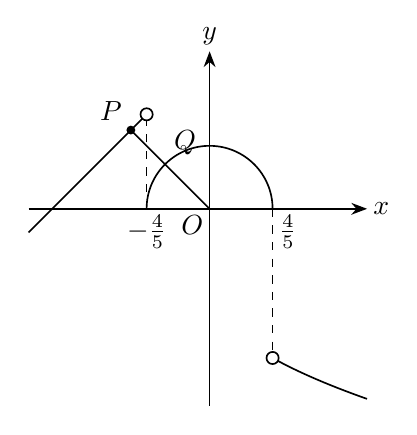
\begin{tikzpicture}[x=1cm,y=1cm,line width=.6pt,>=Stealth,font=\normalsize]
\draw[->] (-2.3,0)--(2.0,0) node[right,inner sep=0pt,xshift=2pt] {$x$};
\draw[->] (0,-2.5)--(0,2.0) node[above,inner sep=0pt,yshift=2pt] {$y$};
\node[below left,inner sep=0pt,xshift=-2pt,yshift=-2pt] at (0,0) {$O$};
\draw[line width=.6pt] (-0.8,0)--(-0.8,0.07);
\draw[line width=.6pt] (0.8,0)--(0.8,0.07);
\node[below,inner sep=0pt,yshift=-2pt] at (-0.8,0) {$-\frac45$};
\node[below right,inner sep=0pt,xshift=2pt,yshift=-2pt] at (0.8,0) {$\frac45$};
% upper semicircle radius 4/5
\draw (-0.8,0) arc[start angle=180,end angle=0,radius=0.8];
% ray y=x+2
\draw (-2.3,-0.3)--(-0.8,1.2);
% descending curve
\draw[domain=0.8:2.0,samples=60] plot (\x,{-sqrt(\x)-1});
% construction diagonal y=-x from P(-1,1) to O
\draw (-1,1)--(0,0);
% dashed droplines
\draw[dashed] (-0.8,0)--(-0.8,1.12);
\draw[dashed] (0.8,0)--(0.8,-1.8144);
% solid P, open endpoints
\fill (-1,1) circle (1.6pt);
\node[above left,inner sep=0pt,xshift=-3pt,yshift=3pt] at (-1,1) {$P$};
% Q label offset perpendicular from diagonal+semicircle (3pt clearance)
\node[above right,inner sep=0pt,xshift=3pt,yshift=3pt] at (-0.56568542,0.56568542) {$Q$};
\draw[fill=white] (-0.8,1.2) circle (2.2pt);
\draw[fill=white] (0.8,-1.89442719) circle (2.2pt);
\end{tikzpicture}
